\subsection{Aplicação Painel: Apagar}
\subsubsection*{Descrição do caso de uso}
Para apagar um registo, o utilizador necessita pressionar o botão \textit{apagar} na linha referente ao registo que pretende atualizar. Pelo facto de ser apenas uma procedimento executado em \textit{background}, não possui nenhuma \textit{view}.

\subsubsection*{\textit{Models} compatíveis com o caso de uso}
Este caso de uso é compatível com os \textit{models} Recolha, Produção, Produto Acabado, Colaboradores, Registo de Ponto, Utilizadores, Pontos de Recolha, Clientes e Analises.

\subsubsection*{Fluxo do caso de utilização}
O caso de uso inicia-se quando o utilizador pressionar o botão apagar da linha do registo que pretende \textit{apagar}. É apresentada uma janela de confirmação. Após executar a ação é apresentada uma mensagem ao utilizador, tal como demonstrado na figura \ref{fig:sd_apagar}


\begin{figure}[H] 
	\begin{center}
		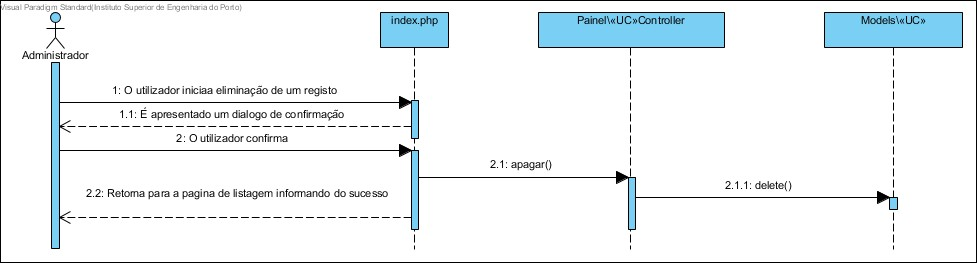
\includegraphics[width=\textwidth,keepaspectratio]{figuras/Diagramas_vp/SD_Painel_4_Apagar.jpg}
		\caption{Diagrama de sequência de apagar registo}
		\label{fig:sd_apagar} 
	\end{center}
\end{figure}